\chapter{Background}

In this seminar project we would be studying the competition neural model for perceptual decision making. Perceptual decision making refers to the decision making of an individual with respect to perception. Studying the neuronal basis of perceptual decision making has found the middle temporal visual area (MT) to respond large motion stimuli. The output of MT region further down the neural pathway activates the Lateral Intra-parietal Area (LIP) before a saccadic eye movement takes place. The LIP neuron activates if a saccadic eye movement would take place in its receptive field. Fig 1 shows the neuronal findings for LIP neurons as reported by Roitman et al \cite{roitman2002response}. Fig A records the response of LIP neurons from the onset of stimuli (triangle) to initiation of saccadic motion. For saccadic motion to the receptive field of the LIP neuron population, we see an increase in firing and a decrease vice versa. The strength of firing depends upon the coherence level of the dots. In fig B. we observe that the saccadic eye motion is initiated only when the neuron reaches a threshold. The threshold is same for different level of coherence. Also, post initiation of the stimuli, there is a dip in the firing rate. Post this dip, the discrimination against for or against the saccadic eye motion takes place.

\begin{figure}
  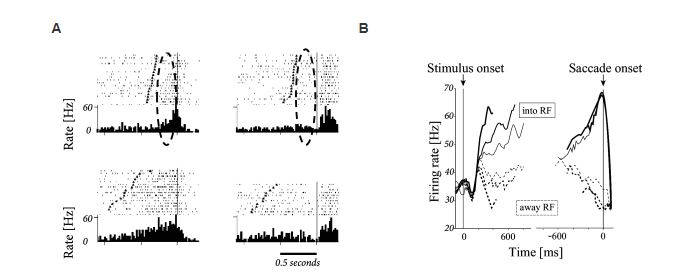
\includegraphics[width=\linewidth]{fig/LIP.jpg}
  \caption{LIP neurons firing to motion discrimination stimuli}
  \label{fig:LIP neuron activity}
\end{figure}

The ramp-to-threshold dynamics of the LIP neurons have been modeled both mathematically and biophysiologically. Shadlen and Newsome \cite{shadlen2001neural} and other scientist have successfully been able to fit the neuronal behaviour to the Diffusion model. However, it leads to a long integration time in decision process making it biologically implausible. 

Likewise, Wang \cite{wang2002probabilistic} was able to replicate the results of Roitman et. al\cite{roitman2002response} and Shadlen et. al \cite{shadlen2001neural} in his biophysically based cortical microcircuit model. However, this model consists of thousands of spiking neurons that interact with each other non linearly. This makes it difficult to analyse the dynamics of the model

This seminar project deals with a reduced version of Wang's model as proposed by Wong et. al \cite{wong2006recurrent}.
